% !TeX program = pdflatex
\documentclass[tikz,border=8pt]{standalone}
\usepackage{pgfplots}\pgfplotsset{compat=1.16}
\definecolor{FigureBlue}{HTML}{2563EB}\definecolor{FigureOrange}{HTML}{EA580C}\definecolor{FigureGreen}{HTML}{16A34A}
\begin{document}
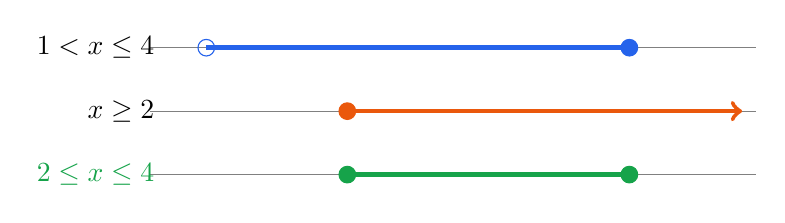
\begin{tikzpicture}
\begin{axis}[width=10cm,height=4.1cm,axis lines=none,xmin=.4,xmax=5.1,ymin=0,ymax=2.5,clip=false]
  \draw[gray] (axis cs:.6,.4)--(axis cs:4.9,.4);
  \draw[gray] (axis cs:.6,1.2)--(axis cs:4.9,1.2);
  \draw[gray] (axis cs:.6,2)--(axis cs:4.9,2);
  \addplot[FigureBlue,ultra thick,no marks] coordinates {(1,2)(4,2)};
  \addplot[FigureOrange,ultra thick,no marks,->] coordinates {(2,1.2)(4.8,1.2)};
  \addplot[FigureGreen,ultra thick,no marks] coordinates {(2,.4)(4,.4)};
  \addplot[only marks,mark=o,mark size=3pt,FigureBlue] coordinates {(1,2)};
  \addplot[only marks,mark=*,mark size=3pt,FigureBlue] coordinates {(4,2)};
  \addplot[only marks,mark=*,mark size=3pt,FigureOrange] coordinates {(2,1.2)};
  \addplot[only marks,mark=*,mark size=3pt,FigureGreen] coordinates {(2,.4)(4,.4)};
  \node[left] at (axis cs:.7,2) {$1<x\le4$};
  \node[left] at (axis cs:.7,1.2) {$x\ge2$};
  \node[left,FigureGreen] at (axis cs:.7,.4) {$2\le x\le4$};
\end{axis}
\end{tikzpicture}
\end{document}
